\documentclass[10pt,twocolumn,letterpaper]{article}
\usepackage[margin=0.75in,columnsep=0.25in]{geometry}
\usepackage{mathptmx}
\usepackage[T1]{fontenc}
\usepackage{microtype}
\usepackage{graphicx}
\usepackage{booktabs}
\usepackage{multirow}
\usepackage{xcolor}
\usepackage{enumitem}
\usepackage{tikz}
\usetikzlibrary{positioning,arrows.meta,decorations.pathreplacing,calc}
\usepackage[hidelinks]{hyperref}
\usepackage[capitalise,noabbrev]{cleveref}
\usepackage{titlesec}
\titlespacing*{\section}{0pt}{6pt plus 2pt}{3pt}
\titlespacing*{\subsection}{0pt}{4pt plus 2pt}{2pt}
\setlist{nosep,leftmargin=*}
\setlength{\textfloatsep}{8pt plus 2pt}
\setlength{\abovecaptionskip}{3pt}
\newcommand{\code}[1]{\texttt{\small #1}}

\title{\Large\bfseries Where Does the GPU Memory Go?\\ Operator-Agnostic Memory Management for TQP-Inmem}
\author{Mingqing Lin\\ University of Michigan}
\date{}

\begin{document}
\maketitle

\begin{abstract}
Tensor Query Processing (TQP) runs SQL on tensor runtimes and is fast on GPUs, but
TQP-Inmem keeps all data in device memory and runs out of memory on a 16\,GB GPU
at TPC-H scale factor (SF)~10. We decompose where the memory goes during a query:
a fixed-block slab pool that never frees during a query, and PyTorch's caching
allocator outside it. With an operator-level trace and exact offline replay, we
find that data no longer needed by any later operator is the largest part of the
slab peak. We implement four memory-management changes that are independent of
any query or operator: last-use reclamation driven by the query plan, coalescing
on every free, a block size planned before execution from a waste budget, and
PyTorch's expandable segments. Results stay identical to the reference.
\end{abstract}

% ---------------------------------------------------------------
\section{Motivation}
\label{sec:motivation}
TQP~\cite{he2022tqp,cui2026tqppp} compiles relational queries into tensor programs
and executes them on tensor runtimes such as PyTorch, which makes GPU query processing
fast without writing custom kernels. TQP-Inmem, the in-memory variant studied here,
keeps every column and intermediate result in GPU memory. Its speed therefore comes with
a hard limit: the data size it can handle is bounded by device memory.
On an RTX~5080 (16\,GB), Q21 fails at SF~10 and Q9 has only about 1\,GB of headroom left
(\cref{fig:ranking}).

This report optimizes how TQP-Inmem \emph{plans and manages} GPU memory, from the
system side, so that it can process queries on larger data. We keep the setting fixed:
a single GPU, all data resident in device memory, results identical to the unmodified
system, and any slowdown reported. All methods are operator-agnostic and query-agnostic:
they depend only on the query plan and the allocator, not on tuning against TPC-H.

% ---------------------------------------------------------------
\section{Background: Memory of One Query}
\label{sec:background}
GPU memory during a TQP-Inmem query has four parts (\cref{fig:layout}).
\begin{itemize}
\item \textbf{CUDA context} ($\approx$0.3\,GB), fixed per process.
\item \textbf{Slab pool.} One \code{torch.empty} byte tensor (4\,GB by default) is
  allocated once and carved into fixed 40\,MB blocks with first-fit placement. Scanned
  columns and every operator output are copied into it. Blocks are only borrowed during
  a query and all are returned at the end (\code{free\_all}).
\item \textbf{PyTorch caching allocator.} Temporaries inside operators (hash tables,
  join candidates, the scan's staging copy) are ordinary PyTorch tensors. Freed tensors
  return to PyTorch's cache (\emph{reserved}), not to the GPU~\cite{pytorchmem}.
\item \textbf{Free device memory.}
\end{itemize}
The split between the slab and PyTorch is \emph{static}: the slab size is chosen at
start-up and neither side can use the other's free space. A query fails in two ways:
the slab has no contiguous run of free blocks (a Python \code{MemoryError}), or PyTorch
cannot obtain device memory (\code{torch.OutOfMemoryError}).

\begin{figure}[t]
\centering
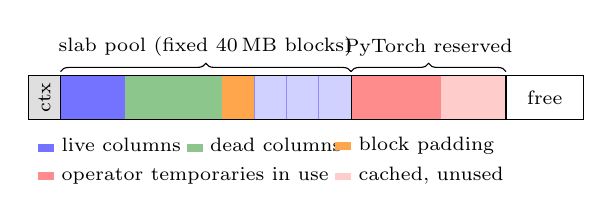
\begin{tikzpicture}[x=0.82cm,y=0.55cm,font=\scriptsize]
  % device bar
  \draw[fill=gray!25] (0,0) rectangle (0.5,1) node[midway,rotate=90]{ctx};
  \draw[fill=blue!18] (0.5,0) rectangle (5,1);
  \foreach \x in {1.0,1.5,...,4.5} \draw[blue!45] (\x,0)--(\x,1);
  \fill[blue!55] (0.5,0) rectangle (1.5,1);
  \fill[green!50!black!45] (1.5,0) rectangle (3.0,1);
  \fill[orange!70] (3.0,0) rectangle (3.5,1);
  \draw (0.5,0) rectangle (5,1);
  \draw[fill=red!20] (5,0) rectangle (7.4,1);
  \fill[red!45] (5,0) rectangle (6.4,1);
  \draw (5,0) rectangle (7.4,1);
  \draw[fill=white] (7.4,0) rectangle (8.6,1) node[midway]{free};
  \draw[decorate,decoration={brace,amplitude=3pt}] (0.5,1.1)--(5,1.1) node[midway,above=2pt]{slab pool (fixed 40\,MB blocks)};
  \draw[decorate,decoration={brace,amplitude=3pt}] (5,1.1)--(7.4,1.1) node[midway,above=2pt]{PyTorch reserved};
  % legend
  \node[anchor=west] at (0,-0.6) {\tikz\fill[blue!55] (0,0) rectangle (0.25,0.18); live columns};
  \node[anchor=west] at (2.3,-0.6) {\tikz\fill[green!50!black!45] (0,0) rectangle (0.25,0.18); dead columns};
  \node[anchor=west] at (4.6,-0.6) {\tikz\fill[orange!70] (0,0) rectangle (0.25,0.18); block padding};
  \node[anchor=west] at (0,-1.3) {\tikz\fill[red!45] (0,0) rectangle (0.25,0.18); operator temporaries in use};
  \node[anchor=west] at (4.6,-1.3) {\tikz\fill[red!20] (0,0) rectangle (0.25,0.18); cached, unused};
\end{tikzpicture}
\caption{GPU memory during one TQP-Inmem query. The slab holds all scanned columns and
operator outputs until the query ends; operator temporaries live in PyTorch's cache.}
\label{fig:layout}
\end{figure}

% ---------------------------------------------------------------
\section{Diagnosis: Why Memory Runs Out}
\label{sec:diagnosis}
We group the possible causes into three ordered categories (\cref{tab:causes}).
The order matters: layout problems depend on which allocations exist and when they
are released, so data and lifetimes must be settled before layout is evaluated.

\begin{table}[t]
\centering\small
\setlength{\tabcolsep}{3pt}
\begin{tabular}{@{}llp{5.1cm}@{}}
\toprule
Category & ID & Cause \\
\midrule
\multirow{2}{*}{Data itself} & S1 & Data that must be resident at the same time (live peak) exceeds the slab \\
 & P2 & Operators create large temporaries outside the slab \\
\midrule
Lifetime & S3 & The slab keeps columns no later operator reads (dead data) \\
\midrule
\multirow{4}{*}{Layout} & S2 & Internal fragmentation: the last block of each allocation is partly empty \\
 & S4 & External fragmentation: free slab blocks are not contiguous \\
 & P1 & PyTorch reserved memory is split across segments \\
 & -- & Static split between slab and PyTorch \\
\bottomrule
\end{tabular}
\caption{Possible causes of out-of-memory failures.}
\label{tab:causes}
\end{table}

\textbf{Data itself.} S1 bounds every storage scheme from below: no layout can go below
the live peak. P2 is the size of operator temporaries, e.g.\ a join that expands
candidate pairs into a dense matrix. Both are reduced only by changing what data is
produced (representation, late materialization~\cite{abadi2007materialization}, or
operator algorithms).

\textbf{Lifetime.} Because the slab never frees during a query, its peak equals the sum
of all scanned columns and all operator outputs. The live data at any moment is
usually much smaller. A reference-counting allocator does not help by itself: every
column stays reachable from the executor's column map (\code{tensor\_group}) until the
plan ends, so it is never \emph{unreachable}, only \emph{unused}. Recognizing it as dead
requires looking ahead in the plan.

\textbf{Layout.} With data and lifetimes fixed, the same bytes can still occupy more
space. In the slab, each allocation is rounded up to whole 40\,MB blocks (S2), and once
blocks are freed mid-query, free runs can be separated by live blocks (S4). In PyTorch,
each \code{cudaMalloc} returns a separate segment and free space in different segments
cannot be combined (P1). Finally, the static split forces each side to reserve for its
own peak even when the two peaks occur at different times.

% ---------------------------------------------------------------
\section{Methodology}
\label{sec:method}
We take the system route: change how memory is planned and managed, without changing
the plan, the operators, or the data representation. This covers S3, S2, S4, P1 and the
static split; S1 and P2 require changing what is computed. For each cause we give
candidate methods and their trade-offs; \cref{sec:impl} describes the ones we built.

\textbf{S3: last-use reclamation.} Freeing needs two answers: \emph{will anyone read
this column later?} and \emph{does anyone still hold this memory now?} Neither alone
saves slab memory. Removing a name from \code{tensor\_group} is always safe (a too-early
removal raises \code{KeyError} at the next lookup) but returns no slab block; reference
counting never fires because the map still holds every column.
\begin{itemize}
\item \emph{Allocator integration.} Make the slab a PyTorch custom allocator so that each
  allocation is its own storage and PyTorch's reference count returns the block. Safety
  holds by construction and temporaries could share the slab, but PyTorch's many small
  tensors would each take a block, the cache would delay returns, and it needs a compiled
  extension.
\item \emph{Executor-level reclamation.} Keep the slab unchanged. After each operator,
  drop the names whose last reader has run, then free every slab allocation that no
  remaining column points to, checked by real device address. Safety rests on one
  checkable invariant: between operators, GPU data is reachable only through
  \code{tensor\_group}, because operators are functions whose locals die on return.
\end{itemize}
The last reader of a column comes from the plan: Spark lists the input columns of every
non-scan operator, and the output operator lists its outputs. This single rule covers all
operator types.

\textbf{S4: coalescing and placement.} Two knobs control holes: \emph{when} adjacent free
runs are merged (the original pool merges after every sixth free) and \emph{where} a new
allocation goes (first-fit, best-fit, or lifetime-aware placement that puts short-lived
data at the high end). Merging only edits a list of a few dozen (start, length) pairs and
moves no data. Lifetime-aware placement needs a threshold for ``short-lived''.

\textbf{S2: block size from a waste budget.} Each allocation wastes less than one block,
so at the peak the internal fragmentation is at most $N\cdot b$, where $N$ is the number of
simultaneously live slab allocations and $b$ the block size. $N$ is a property of the plan
(it is identical at SF~5 and SF~10). Given the slab capacity $P$ and a tolerated waste
fraction $\varepsilon$, we choose the largest $b$ with $N\cdot b \le \varepsilon P$ before
the query runs. The only parameter, $\varepsilon$, has a direct meaning. A fixed tiny
granularity removes the parameter but decouples the block from any transfer unit.

\textbf{P1: PyTorch segments.} PyTorch already merges adjacent free blocks immediately
and uses best-fit, so its remaining fragmentation comes from segment boundaries.
\emph{Expandable segments}~\cite{pytorchmem} reserve one large virtual range and map
physical pages on demand; fully free pages can be unmapped and remapped elsewhere, so
holes cost virtual addresses rather than device memory, the same idea as paging in
PagedAttention~\cite{kwon2023paged}. Mapping changes page tables only and moves no data,
but growing a segment may take several driver calls. Calling \code{empty\_cache} after
every operator returns fully free segments instead, at the cost of re-allocating them.

\textbf{Static split.} The total need under a static split is the slab peak plus the
PyTorch peak, while a shared space needs only the maximum over time of their sum.
Two ways close the gap: let PyTorch temporaries allocate from the slab (the allocator
integration above), or size the slab to the post-reclamation need so that its savings
go to PyTorch.

% ---------------------------------------------------------------
\section{Implementation}
\label{sec:impl}
% TODO(claude): fill after code review

% ---------------------------------------------------------------
\section{Experiments}
\label{sec:exp}
% TODO(claude): fill with results

\begin{figure}[t]
\centering
% \includegraphics[width=\columnwidth]{figures/ranking.png}
\caption{Total GPU need per query at SF~10 (slab peak + PyTorch peak + context), sorted;
dashed line: device capacity.}
\label{fig:ranking}
\end{figure}

% ---------------------------------------------------------------
\section{Results}
\label{sec:results}

% ---------------------------------------------------------------
\section{Trade-offs}
\label{sec:tradeoffs}

% ---------------------------------------------------------------
\section{Reproduction}
\label{sec:repro}

\small
\bibliographystyle{plain}
\bibliography{refs}
\end{document}
